\documentclass{standalone}
\usepackage{tikz}
\usetikzlibrary{shapes.geometric, arrows}

%Inicio del preambulo

\tikzstyle{startstop} = [rectangle, rounded corners, minimum width=3cm, minimum height=1cm,text centered, draw=black, fill=red!30]

\tikzstyle{io} = [trapezium, trapezium left angle=70, trapezium right angle=110, minimum width=3cm, minimum height=1cm, text centered, draw=black, fill=blue!30]

\tikzstyle{process} = [rectangle, minimum width=3cm, minimum height=1cm, text centered, draw=black, fill=orange!30]

\tikzstyle{decision} = [diamond, minimum width=3cm, minimum height=1cm, text centered, draw=black, fill=green!30]

\tikzstyle{arrow} = [thick,->,>=stealth]

%Fin del preambulo

\begin{document}

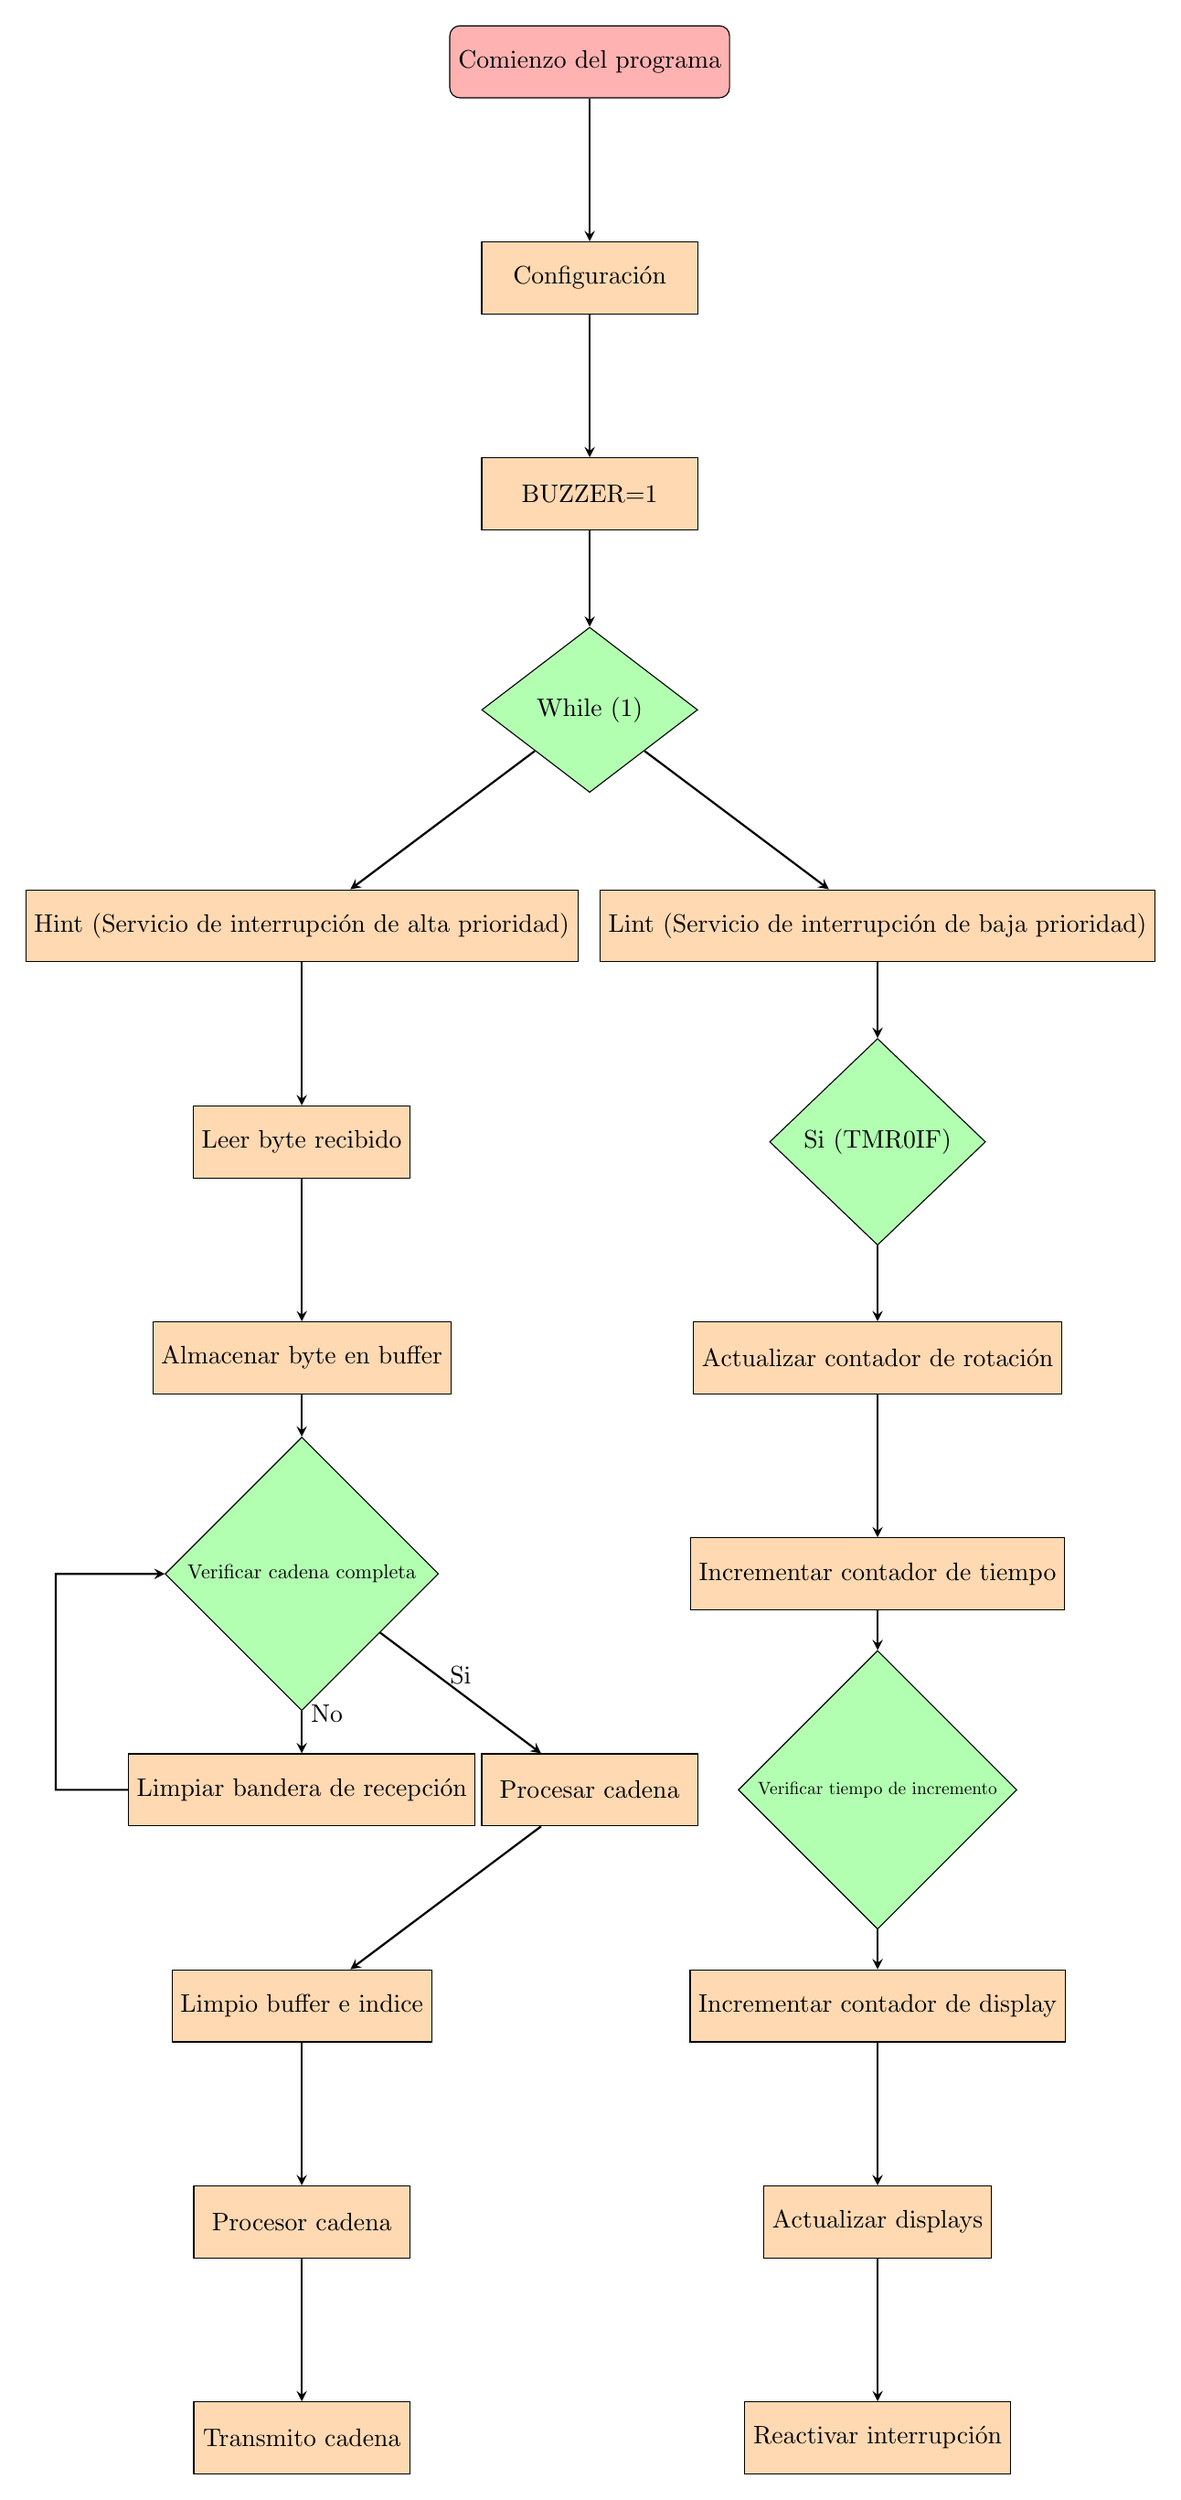
\begin{tikzpicture}[node distance=3cm]

\node (start) [startstop] {Comienzo del programa};
\node (config) [process, below of=start] {Configuración};
\node (buzzer) [process, below of=config] {BUZZER=1};
\node (while) [decision, below of=buzzer] {While (1)};

\node (hint) [process, below of=while, xshift=-4cm] {Hint (Servicio de interrupción de alta prioridad)};
\node (leer) [process, below of=hint] {Leer byte recibido};
\node (almacenar) [process, below of=leer] {Almacenar byte en buffer};
\node (verificar) [decision, below of=almacenar, scale=0.8] {Verificar cadena completa};
\node (procesar) [process, below of=verificar, xshift=4cm] {Procesar cadena};
\node (limpiar) [process, below of=verificar] {Limpiar bandera de recepción};

\node (lint) [process, below of=while, xshift=4cm] {Lint (Servicio de interrupción de baja prioridad)};
\node (t0if) [decision, below of=lint] {Si (TMR0IF)};
\node (actualizar) [process, below of=t0if] {Actualizar contador de rotación};
\node (incrementar) [process, below of=actualizar] {Incrementar contador de tiempo};
\node (verificar2) [decision, below of=incrementar,scale=0.7] {Verificar tiempo de incremento};
\node (incrementar2) [process, below of=verificar2] {Incrementar contador de display};
\node (actualizar2) [process, below of=incrementar2] {Actualizar displays};
\node (reactivar) [process, below of=actualizar2] {Reactivar interrupción};

\node (bufclean) [process, below of=procesar, xshift=-4cm] {Limpio buffer e indice};
\node (netwprocss) [process, below of=bufclean] {Procesor cadena};
\node (netwtrans) [process, below of=netwprocss] {Transmito cadena};

\draw [arrow] (start) -- (config);
\draw [arrow] (config) -- (buzzer);
\draw [arrow] (buzzer) -- (while);
\draw [arrow] (while) -- (hint);
\draw [arrow] (while) -- (lint);
\draw [arrow] (hint) -- (leer);
\draw [arrow] (leer) -- (almacenar);
\draw [arrow] (almacenar) -- (verificar);
\draw [arrow] (verificar) --node[anchor=south]{Si} (procesar);
\draw [arrow] (verificar) --node[anchor=south west]{No} (limpiar);
\draw [arrow] (limpiar.west) --++(-1,0)--++(0,3)-- (verificar.west);
\draw [arrow] (lint) -- (t0if);
\draw [arrow] (t0if) -- (actualizar);
\draw [arrow] (actualizar) -- (incrementar);
\draw [arrow] (incrementar) -- (verificar2);
\draw [arrow] (verificar2) -- (incrementar2);
\draw [arrow] (incrementar2) -- (actualizar2);
\draw [arrow] (actualizar2) -- (reactivar);
\draw [arrow] (procesar) -- (bufclean);
\draw [arrow] (bufclean) -- (netwprocss);
\draw [arrow] (netwprocss) -- (netwtrans);

\end{tikzpicture}

\end{document}